\documentclass[11pt]{article}
\usepackage{tikz}
\usepackage{amsmath}
\usetikzlibrary{calc, shapes, backgrounds}
\author{Parham Alvani}
\title{Computer Architecture Homework 1}
\begin{document}
\begin{titlepage}
\begin{center}
\emph{In The Name of God}
\end{center}
\maketitle
\begin{center}
powered by \LaTeX
\end{center}
\end{titlepage}
\tableofcontents
\newpage
\section{Problem 2}
\paragraph{1}
\paragraph{2}
According to following diagram :

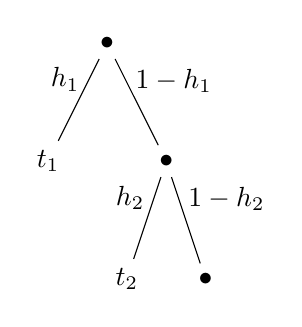
\begin{tikzpicture}[level 2/.style={sibling distance=10mm}]
	\node (START) {$\bullet$}
		child { node (T1) {$t_1$}}
		child { node (@T1) {$\bullet$}
			child {node (T2) {$t_2$}}
			child {node (@T2) {$\bullet$}}
		};
	\begin{scope}[nodes = {draw = none}]
		\path (START) -- (T1)  node [near start, left]  {$h_1$};
    		\path (START) -- (@T1) node [near start, right] {$1 - h_1$};
		\path (@T1)   -- (T2)  node [near start, left]  {$h_2$};
		\path (@T1)   -- (@T2) node [near start, right] {$1 - h_2$};
	\end{scope}
\end{tikzpicture}

\begin{itemize}
\item
	Average Memory Access Time, the exact formula
	\begin{equation}
		\label{eq:AMAT-e}
	\end{equation}	
\item
	Average Memory Access Time, an approximate formula
	\begin{equation}
		\label{eq:AMAT-a}
		h_1 * t_1 + (1 - h_1) [h_2 * t_2 + (1 - h_2)(\ldots)]
	\end{equation}
\end{itemize}
\paragraph{3}
\paragraph{4}
\paragraph{5}
\section{Problem 3}
The following is the avrage memory access time equlation for
memory with 3 level:
\begin{equation}
	\label{eq:AMAT-3}
	\bar{T} = h_1 * t_1 + (1 - h_1) * h_2 * t_2 + (1 - h_1) * (1 - h_2) * h_3 * t_3
\end{equation}
Substituting $1ns$ for $t_1$, $0.1$ for $h_1$, $10ns$ for $t_2$, $0.5$ for $h_2$, $1000ns$ for $t_3$ and $1$ for $h_3$
in (\ref{eq:AMAT-3}) gives us:
\begin{align*}
	\bar{T} = 0.1 * 1 + (1 - 0.1) * 0.5 * 10 + (1 - 0.1) * (1 - 0.5) * 1000\\
	= 0.1 + 0.9 * 0.5 * 10 + 0.9 * 0.5 * 1000\\
	= 0.10 + 0.45 * 10 + 0.45 * 1000\\
	= 0.10 + 4.50 + 450.00\\
	= 454.60ns
\end{align*}
\section{Problem 4}
The following is the avrage memory access time equlation for
memory with 4 level:
\begin{equation}
	\label{eq:AMAT-4}
	\bar{T} = h_1 * t_1 + (1 - h_1) * h_2 * t_2 + (1 - h_1) * (1 - h_2) * h_3 * t_3 + (1 - h_1) * (1 - h_2) * (1 - h_3) * h_4 * t_4
\end{equation}
Substituting $1ns$ for $t_1$, $0.1$ for $h_1$, $10ns$ for $t_2$, $0.5$ for $h_2$, $8s$ for $t_3$, $0.63$ for $h_3$,$1000ns$ for $t_4$, $1$ for $h_3$,
in (\ref{eq:AMAT-4}) gives us:
\begin{align*}
	\bar{T} &= 0.1 * 1 + (1 - 0.1) * 0.5 * 10 + (1 - 0.1) * (1 - 0.5) * 0.63 * 8 + \\
	&\qquad \phantom{= 0.1 * 1 + (1 - 0.1)} (1 - 0.1) * (1 - 0.5) * (1 - 0.63) * 1000 \\
	&= 0.1 * 1 + 0.9 * 0.5 * 10 + 0.9 * 0.5 * 0.63 * 8 + 0.9 * 0.5 * 0.37 * 1000 \\
	&= 0.10 + 0.45 * 10 + 0.28 * 8 + 0.16 * 1000 \\
	&= 0.10 + 4.50 + 2.24 + 160.00 \\
	&= 166.84ns
\end{align*}
\section{Problem 5}
\paragraph{1}
Adrress bits $= 14$ bits, \qquad Length $= 2$ bytes, \qquad Width $= 2^{14}$ words, \qquad The smallest unit available $= 16$ bits.
\paragraph{2}
Adrress bits $= 15$ bits, \qquad Length $= 2$ bytes, \qquad Width $= 2^{15}$ words, \qquad The smallest unit available $= 16$ bits.
\paragraph{3}
Adrress bits $= 15$ bits, \qquad Length $= 1$ bytes, \qquad Width $= 2^{15}$ words, \qquad The smallest unit available $= 8$ bits.
\paragraph{4}
Adrress bits $= 13$ bits, \qquad Length $= 4$ bytes, \qquad Width $= 2^{13}$ words, \qquad The smallest unit available $= 32$ bits.
\end{document}
